\documentclass[10pt,ignorenonframetext,,aspectratio=149]{beamer}
\usefonttheme{serif} % use mainfont rather than sansfont for slide text
\setbeamertemplate{caption}[numbered]
\setbeamertemplate{caption label separator}{: }
\setbeamercolor{caption name}{fg=normal text.fg}
\usepackage{lmodern}
\usepackage{amssymb,amsmath}
\usepackage{ifxetex,ifluatex}
\usepackage{fixltx2e} % provides \textsubscript
\ifnum 0\ifxetex 1\fi\ifluatex 1\fi=0 % if pdftex
  \usepackage[T1]{fontenc}
  \usepackage[utf8]{inputenc}
\else % if luatex or xelatex
  \ifxetex
    \usepackage{mathspec}
  \else
    \usepackage{fontspec}
  \fi
  \defaultfontfeatures{Ligatures=TeX,Scale=MatchLowercase}
  \newcommand{\euro}{€}
    \setmainfont[]{Open Sans}
\fi
% use upquote if available, for straight quotes in verbatim environments
\IfFileExists{upquote.sty}{\usepackage{upquote}}{}
% use microtype if available
\IfFileExists{microtype.sty}{%
\usepackage{microtype}
\UseMicrotypeSet[protrusion]{basicmath} % disable protrusion for tt fonts
}{}
\usepackage{graphicx,grffile}
\makeatletter
\def\maxwidth{\ifdim\Gin@nat@width>\linewidth\linewidth\else\Gin@nat@width\fi}
\def\maxheight{\ifdim\Gin@nat@height>\textheight0.8\textheight\else\Gin@nat@height\fi}
\makeatother
% Scale images if necessary, so that they will not overflow the page
% margins by default, and it is still possible to overwrite the defaults
% using explicit options in \includegraphics[width, height, ...]{}
\setkeys{Gin}{width=\maxwidth,height=\maxheight,keepaspectratio}

% Comment these out if you don't want a slide with just the
% part/section/subsection/subsubsection title:
\AtBeginPart{
  \let\insertpartnumber\relax
  \let\partname\relax
  \frame{\partpage}
}
\AtBeginSection{
  \let\insertsectionnumber\relax
  \let\sectionname\relax
  \frame{\sectionpage}
}
\AtBeginSubsection{
  \let\insertsubsectionnumber\relax
  \let\subsectionname\relax
  \frame{\subsectionpage}
}

\setlength{\emergencystretch}{3em}  % prevent overfull lines
\providecommand{\tightlist}{%
  \setlength{\itemsep}{0pt}\setlength{\parskip}{0pt}}
\setcounter{secnumdepth}{0}

\title{Models of Panel Data}
\author{Henrique Veras}
\date{}

%% Here's everything I added.
%%--------------------------

\usepackage{graphicx}
\usepackage{rotating}
%\setbeamertemplate{caption}[numbered]
\usepackage{hyperref}
\usepackage{caption}
\usepackage[normalem]{ulem}
%\mode<presentation>
\usepackage{wasysym}
%\usepackage{amsmath}


% Get rid of navigation symbols.
%-------------------------------
\setbeamertemplate{navigation symbols}{}

% Optional institute tags and titlegraphic.
% Do feel free to change the titlegraphic if you don't want it as a Markdown field.
%----------------------------------------------------------------------------------
\institute{PIMES/UFPE}

% \titlegraphic{\includegraphics[width=0.3\paperwidth]{\string~/Dropbox/teaching/clemson-academic.png}} % <-- if you want to know what this looks like without it as a Markdown field. 
% -----------------------------------------------------------------------------------------------------


% Some additional title page adjustments.
%----------------------------------------
\setbeamertemplate{title page}[empty]
%\date{}
\setbeamerfont{subtitle}{size=\small}

\setbeamercovered{transparent}

% Some optional colors. Change or add as you see fit.
%---------------------------------------------------
\definecolor{clemsonpurple}{HTML}{522D80}
 \definecolor{clemsonorange}{HTML}{F66733}
\definecolor{uiucblue}{HTML}{003C7D}
\definecolor{uiucorange}{HTML}{F47F24}


% Some optional color adjustments to Beamer. Change as you see fit.
%------------------------------------------------------------------
\setbeamercolor{frametitle}{fg=clemsonpurple,bg=white}
\setbeamercolor{title}{fg=clemsonpurple,bg=white}
\setbeamercolor{local structure}{fg=clemsonpurple}
\setbeamercolor{section in toc}{fg=clemsonpurple,bg=white}
% \setbeamercolor{subsection in toc}{fg=clemsonorange,bg=white}
\setbeamercolor{footline}{fg=clemsonpurple!50, bg=white}
\setbeamercolor{block title}{fg=clemsonorange,bg=white}


\let\Tiny=\tiny


% Sections and subsections should not get their own damn slide.
%--------------------------------------------------------------
\AtBeginPart{}
\AtBeginSection{}
\AtBeginSubsection{}
\AtBeginSubsubsection{}

% Suppress some of Markdown's weird default vertical spacing.
%------------------------------------------------------------
\setlength{\emergencystretch}{0em}  % prevent overfull lines
\setlength{\parskip}{0pt}


% Allow for those simple two-tone footlines I like. 
% Edit the colors as you see fit.
%--------------------------------------------------
\defbeamertemplate*{footline}{my footline}{%
    \ifnum\insertpagenumber=1
    \hbox{%
        \begin{beamercolorbox}[wd=\paperwidth,ht=.8ex,dp=1ex,center]{}%
      % empty environment to raise height
        \end{beamercolorbox}%
    }%
    \vskip0pt%
    \else%
        \Tiny{%
            \hfill%
		\vspace*{1pt}%
            \insertframenumber/\inserttotalframenumber \hspace*{0.1cm}%
            \newline%
            \color{clemsonpurple}{\rule{\paperwidth}{0.4mm}}\newline%
            \color{clemsonorange}{\rule{\paperwidth}{.4mm}}%
        }%
    \fi%
}

% Various cosmetic things, though I must confess I forget what exactly these do and why I included them.
%-------------------------------------------------------------------------------------------------------
\setbeamercolor{structure}{fg=blue}
\setbeamercolor{local structure}{parent=structure}
\setbeamercolor{item projected}{parent=item,use=item,fg=clemsonpurple,bg=white}
\setbeamercolor{enumerate item}{parent=item}

% Adjust some item elements. More cosmetic things.
%-------------------------------------------------
\setbeamertemplate{itemize item}{\color{clemsonpurple}$\bullet$}
\setbeamertemplate{itemize subitem}{\color{clemsonpurple}\scriptsize{$\bullet$}}
\setbeamertemplate{itemize/enumerate body end}{\vspace{.6\baselineskip}} % So I'm less inclined to use \medskip and \bigskip in Markdown.

% Automatically center images
% ---------------------------
% Note: this is for ![](image.png) images
% Use "fig.align = "center" for R chunks

\usepackage{etoolbox}

\AtBeginDocument{%
  \letcs\oig{@orig\string\includegraphics}%
  \renewcommand<>\includegraphics[2][]{%
    \only#3{%
      {\centering\oig[{#1}]{#2}\par}%
    }%
  }%
}

% I think I've moved to xelatex now. Here's some stuff for that.
% --------------------------------------------------------------
% I could customize/generalize this more but the truth is it works for my circumstances.

\ifxetex
\setbeamerfont{title}{family=\fontspec{Titillium Web}}
\setbeamerfont{frametitle}{family=\fontspec{Titillium Web}}
\usepackage[font=small,skip=0pt]{caption}
 \else
 \fi

% Okay, and begin the actual document...

\begin{document}
\frame{\titlepage}

\hypertarget{econometrics}{%
\section{Econometrics}\label{econometrics}}

\hypertarget{intro}{%
\subsection{Intro}\label{intro}}

\begin{frame}{Intro}
Here we will study models that deal with data sets that combine time
series and cross sections: \textbf{panel data sets}.

\vfill

The analysis of panel data allows us to learn about the economic
processes while accounting for both \textbf{heterogeneity} across units
of observations and for the dynamic effects that are not visible in
cross-secions.

\vfill
\end{frame}

\hypertarget{panel-data-modeling}{%
\subsection{Panel Data Modeling}\label{panel-data-modeling}}

\begin{frame}{Panel Data Modeling}
Panel data models are more oriented toward cross-section analyses

\begin{itemize}
\tightlist
\item
  they are wide but typically short.
\end{itemize}

\vfill

Thus, in the typical panel, there are a large number of cross-sectional
units and only a few periods.

\vfill
\end{frame}

\begin{frame}{The General Modeling Framework for Analyzing Panel Data}
\protect\hypertarget{the-general-modeling-framework-for-analyzing-panel-data}{}
The basic framework is a regression model of the form

\[\begin{split} y_{it} = & \mathbf{x}_{it}'\pmb{\beta}+\mathbf{z}_i'\pmb{\alpha}+\varepsilon_{it}\\
 = & \mathbf{x}_{it}'\pmb{\beta}+ c_i+\varepsilon_{it} \end{split}\]

There are \(K\) regressors in \(\mathbf{x}_{it}\), not including the
constant term.

\vfill

The heterogeneity, or individual effect, is
\(\mathbf{z}_i'\pmb{\alpha}\) where \(\mathbf{z}_i\) contains a constant
term and a set of individual or group-specific variables, which may be
observed, such as race, sex, location, and so on; or unobserved, such as
family specific characteristics, individual heterogeneity in skill or
preferences, and so on, all of which are taken to be constant over time
\(t\).

\vfill
\end{frame}

\begin{frame}{The General Modeling Framework for Analyzing Panel Data}
\protect\hypertarget{the-general-modeling-framework-for-analyzing-panel-data-1}{}
Notice that if all variables in \(\mathbf{z}\) are observable, we could
estimate the model above by OLS.

\vfill

The complication, however, arises when \(c_i\) is \textbf{unobserved}.

\vfill

Our main objective here will be consistent and efficient estimation of
the \textbf{partial effects}

\[\mathbf{\pmb{\beta}}=\partial E[y_{it}|\mathbf{x}_{it}]/\partial \mathbf{x}_{it} \]

\vfill

Whether this is possible depends on the assumptions about the unobserved
(latent) effects.

\vfill
\end{frame}

\begin{frame}{The General Modeling Framework for Analyzing Panel Data}
\protect\hypertarget{the-general-modeling-framework-for-analyzing-panel-data-2}{}
We can begin with a \textbf{strict exogeneity} assumption for the
independent variables,

\[E[\varepsilon_{it}|\mathbf{x}_{i1},\mathbf{x}_{i2},\ldots,c_i]=E[\varepsilon_{it}|\mathbf{X}_i,c_i]=0\]

This implies that the current disturbance is uncorrelated with the
independent variables in every period, past, present, and future.

\vfill

This assumption is sometimes unnecessarily strong but it is a convenient
starting point and useful in some applications.

\vfill
\end{frame}

\begin{frame}{The General Modeling Framework for Analyzing Panel Data}
\protect\hypertarget{the-general-modeling-framework-for-analyzing-panel-data-3}{}
A looser assumption of contemporaneous exogeneity is sometimes useful:

\[E[\varepsilon_{it}|\mathbf{x}_{it},c_i]=0\]

\vfill

The regression model with this assumption restricts influences of
\(\mathbf{x}\) on \(E[\mathbf{y}|\mathbf{x}, c]\) to the current period.

\vfill
\end{frame}

\begin{frame}{The General Modeling Framework for Analyzing Panel Data}
\protect\hypertarget{the-general-modeling-framework-for-analyzing-panel-data-4}{}
The crucial aspect of the model concerns the heterogeneity.

\vfill

A conventional assumption is the \textbf{mean independence},

\[E[c_i|\mathbf{x}_{i1},\mathbf{x}_{i2},\ldots,]=\alpha\] This
assumption, which underlines the \emph{random effects} model that we
will discuss later, states that the unobserved variables are
uncorrelated with the included variables.

\vfill

This is also a strong assumption and likely to be violated in many
empirical applications.

\vfill

A weaker assumption would be that
\(E[c_i|\mathbf{x}_{i1},\mathbf{x}_{i2},\ldots,]=h(\mathbf{x}_{i1},\mathbf{x}_{i2},\ldots,)=h(\mathbf{X}_i)\)
for some unspecified but nonconstant function of \(\mathbf{X}_i\).

\vfill
\end{frame}

\begin{frame}{Model Structures}
\protect\hypertarget{model-structures}{}
Panel data models can broadly be arranged as follows:

\begin{enumerate}
\tightlist
\item
  \textbf{Pooled regression}: If \(\mathbf{z}_i\) contains only a
  constant term, then the OLS estimator provides consistent and
  efficient estimates of the common \(\alpha\) and slope vector
  \(\pmb{\beta}\).
\item
  \textbf{Fixed effects}: If \(\mathbf{z}_i\) is unobserved, but
  correlated with \(\mathbf{x}_{it}\), then the OLS estimator of
  \(\pmb{\beta}\) is biased and inconsistent (why?). However, the model
  \[y_{it}=\mathbf{x}_{it}'\pmb{\beta}+ \alpha_i+\varepsilon_{it},\]
  where \(\alpha_i=\mathbf{z}_i'\alpha\) embodies all the observable
  effects and specifies an estimable conditional mean.
\end{enumerate}

\vfill
\end{frame}

\begin{frame}{Model Structures}
\protect\hypertarget{model-structures-1}{}
Panel data models can broadly be arranged as follows:

\begin{enumerate}
\setcounter{enumi}{2}
\tightlist
\item
  \textbf{Random effects}: If the observed individual heterogeneity is
  uncorrelated with \(\mathbf{x}_{it}\), the model may be formulated as
\end{enumerate}

\[\begin{split} y_{it} = & \mathbf{x}_{it}'\beta+E[\mathbf{z}_i'\alpha]+ \mathbf{z}_i'\alpha-E[\mathbf{z}_i'\alpha]+\varepsilon_{it}\\
   = & \mathbf{x}_{it}'\beta + \alpha + u_i + \varepsilon_{it}  \end{split}\]

that is, a linear regression model with a compound disturbance that may
consistently, albeit inefficiently, estimated by LS.
\end{frame}

\begin{frame}{Balanced and Unbalanced Panels}
\protect\hypertarget{balanced-and-unbalanced-panels}{}
As suggested by the preceding discussion, a panel data set consists of
\(n\) set of observations on individuals.

\vfill

If each individual is observed the same number of times \(T\), the data
set is a \textbf{balanced panel}.

\vfill

An \textbf{unbalanced panel} data set is one in which individuals may be
observed different number of times.

\begin{itemize}
\tightlist
\item
  In empirical applications, this might be due to \textbf{attrition}.
\end{itemize}

\vfill

A \textbf{fixed panel} is one in which the same set of individuals is
observed for the duration of the study.

\vfill

A \textbf{rotating panel} is one in which the cast of individuals
changes from one period to the next.

\vfill
\end{frame}

\begin{frame}{Well-Behaved Panel Data}
\protect\hypertarget{well-behaved-panel-data}{}
Throughout the analysis we consider assumptions A.1. through A.4., as
well as the asymptotic conditions on the matrices \(\mathbf{X'X}/n\) and
\((\mathbf{X}'\pmb{\varepsilon})/n\).

\vfill

Exceptions to the assumptions are likely to arise in a panel data set.

\begin{itemize}
\tightlist
\item
  For example, the \(\mathbf{x}_i\)'s may be correlated across
  observations as they might be the same individual observed in multiple
  periods.
\end{itemize}

\vfill
\end{frame}

\begin{frame}{Well-Behaved Panel Data}
\protect\hypertarget{well-behaved-panel-data-1}{}
The panel data set could be treated as follows:

\begin{itemize}
\tightlist
\item
  Since the total number of rows in \(\mathbf{X}\) is now
  \(N=n\times T\), the matrix \(\bar{\mathbf{Q}}_n\) is
\end{itemize}

\[\bar{\mathbf{Q}}_n=\frac{1}{n}\sum_{i=1}^n{\frac{1}{T}\mathbf{X_i'X_i}}=\frac{1}{n}\sum_{i=1}^n{\mathbf{Q}_i}\]

\vfill

We then view the set of observations on the \(i\)th unit as if they were
a single observation and apply our convergence arguments to the number
of units increasing without bound.

\vfill
\end{frame}

\hypertarget{the-pooled-regression-model}{%
\subsection{The Pooled Regression
Model}\label{the-pooled-regression-model}}

\begin{frame}{The Pooled Regression Model}
The simplest version of the model assumes

\[y_{it}= \alpha + \mathbf{x}_{it}'\beta+\varepsilon_{it}, i=1,\ldots,n; t=1,\ldots,T_i\]

\[E[\varepsilon_{it}|\mathbf{x}_{i1},\mathbf{x}_{i2},\ldots,\mathbf{x}_{iT_i}]=0\]

\[E[\varepsilon_{it}\varepsilon_{js}|\mathbf{x}_{i1},\mathbf{x}_{i2},\ldots,\mathbf{x}_{iT_i}]=\sigma_\varepsilon^2 \text{ if } i=j \text{ and } t=s \text{ and } = 0 \text{ if } i\neq j \text{ or } t\neq s  \]

\vfill
\end{frame}

\begin{frame}{Least Squares Estimation of the Pooled Model}
\protect\hypertarget{least-squares-estimation-of-the-pooled-model}{}
In the form above, if the remaining assumptions of the classical model
are met, then no further analysis is needed.

\vfill

OLS is the efficient estimator and inference can reliably proceed along
the lines of the methods developed earlier in the course.

\vfill

The question, then, is what can be expected of the estimator when the
heterogeneity does differ across individuals?

\vfill

The fixed effects case is obvious: omitting (or ignoring) the
heterogeneity when the fixed effects model is appropriate renders the
least squares estimator inconsistent---sometimes wildly so. In the
random effects case, the unobserved heterogeneity induces
autocorrelation.

\vfill
\end{frame}

\begin{frame}{Robust Covariance Matrix}
\protect\hypertarget{robust-covariance-matrix}{}
Suppose we stack the \(T_i\) observations for individual \(i\) in a
single equation

\[\mathbf{y}_i=\mathbf{x}_i\beta + \mathbf{w}_i\]

In a panel data set, although heteroskedasticity might be present, the
more substantive effect is cross-observation correlation (or
autocorrelation).

\vfill

The group of observations may all pertain to the same individual, so any
latent effects left out of the model will carry across all periods.

\vfill

Let's assume that the disturbances vector consists of
\(\varepsilon_{it}\) plus an omitted individual component. Then,

\[\begin{split}Var[\mathbf{w}_i|\mathbf{X}_i] = & \sigma_\varepsilon^2\mathbf{I}_{T_i}+\mathbf{\Sigma}_i\\
  = & \mathbf{\Omega}_i \end{split}\]

\vfill
\end{frame}

\begin{frame}{Robust Covariance Matrix}
\protect\hypertarget{robust-covariance-matrix-1}{}
The OLS estimator of \(\mathbf{\beta}\) is

\[\begin{split} \mathbf{b} = & (\mathbf{X'X})^{-1}\mathbf{X'y} \\
 = & \pmb{\beta} + \left[\sum_{i=1}^n{\mathbf{X_i'X_i}} \right]^{-1}\sum_{i=1}^n{\mathbf{X}_i'\mathbf{w}_i}  \end{split}\]

Consistency of \(\mathbf{b}\) can be established as before.

\vfill

The true covariance matrix would take the form we saw for the GLS model

\[Asy.Var[\mathbf{b}]=\frac{1}{n}\text{plim }\left[\frac{1}{n} \sum_{i=1}^n{\mathbf{X_i'X_i}} \right]^{-1}\text{plim }\left[\sum_{i=1}^n{\mathbf{X}_i '\mathbf{\Omega}_i\mathbf{X}_i} \right]\text{plim }\left[\frac{1}{n} \sum_{i=1}^n{\mathbf{X_i'X_i}} \right]^{-1}\]

As before, the center matrix must be estimated.

\vfill
\end{frame}

\begin{frame}{Robust Covariance Matrix}
\protect\hypertarget{robust-covariance-matrix-2}{}
We can estimate \(Asy.Var[\mathbf{b}]\) with

\[Est.Asy.Var[\mathbf{b}]=\frac{1}{n}\text{plim }\left[\frac{1}{n} \sum_{i=1}^n{\mathbf{X_i'X_i}} \right]^{-1}\text{plim }\left[\sum_{i=1}^n{\mathbf{X}_i '\mathbf{\hat{w}\hat{w}}_i'\mathbf{X}_i} \right]\text{plim }\left[\frac{1}{n} \sum_{i=1}^n{\mathbf{X_i'X_i}} \right]^{-1}\]

where \(\mathbf{\hat{w}}_i\) is the vector of \(T_i\) residuals for
individual \(i\).

\vfill

This construction is analogous to the ``cluster''-robust estimator
developed earlier.

\vfill
\end{frame}

\begin{frame}{Robust Estimation Using Group Means}
\protect\hypertarget{robust-estimation-using-group-means}{}
The pooled regression model can also be estimated using the sample means
of the data.

\vfill

Pre-multiplying the regression model by \((1/T)\mathbf{i}'\), where
\(\mathbf{i}'\) is a row vector of ones,

\[(1/T)\mathbf{i}'\mathbf{y}_i=(1/T)\mathbf{i'x_i}\pmb{\beta}+(1/T)\mathbf{i'w}_i\]

or

\[\bar{y}_i=\mathbf{\bar{x}}_i'\pmb{\beta}+\bar{w}_i\]

Heteroskedastic variances are now
\(\sigma_i^2=(1/T^2)\mathbf{i}'\mathbf{\Omega_ii}\).

\vfill
\end{frame}

\begin{frame}{Robust Estimation Using Group Means}
\protect\hypertarget{robust-estimation-using-group-means-1}{}
Consider, on the other hand, the general model

\[\mathbf{y}_i= \mathbf{x_i}\pmb{\beta}+c_i\mathbf{i}+\mathbf{w}_i,\]

where \(c_i\) is the (latent) heterogeneous effect.

\vfill

If the mean independence assumption, \(E[c_i|\mathbf{X}_i]=\alpha\) is
not met, then the effect will be transmitted to the group means as well.

\vfill

Averaging the observations in the group collects the entire set of
effects, observed and latent, in the group means. Therefore, estimating
\(\pmb{\beta}\) by OLS will be both biased and inconsistent.

\vfill
\end{frame}

\begin{frame}{Estimator with First Differences}
\protect\hypertarget{estimator-with-first-differences}{}
First differencing is another approach to estimation.

\vfill

Consider the model

\[y_{it} = c_i+ \mathbf{x}_{it}'\pmb{\beta}+\varepsilon_{it}\]

which implies the first differences equation

\[\Delta y_{it} = \Delta c_i + (\Delta \mathbf{x}_{it})'\pmb{\beta} + \Delta \varepsilon_{it} \]

or

\[\begin{split} \Delta y_{it} = &  (\Delta \mathbf{x}_{it})'\pmb{\beta} + \varepsilon_{it} - \varepsilon_{i,t-1}\\
 = & (\Delta \mathbf{x}_{it})'\pmb{\beta} + u_{it}
\end{split}\]
\end{frame}

\begin{frame}{Estimator with First Differences}
\protect\hypertarget{estimator-with-first-differences-1}{}
The advantage of the first difference approach is that it removes the
heterogeneity from the model.

\vfill

The disadvantage is that it removes all time-invariant variables from
the model.

\begin{itemize}
\tightlist
\item
  If we have a panel data set and want to estimate the effects of
  schooling on wages, for example, we would not be able to employ this
  strategy, as years of education of workers are usually fixed in time.
\end{itemize}

\vfill

Note as well that the differencing procedure trades the
cross-observation correlation in \(c_i\) for a moving average (MA)
disturbances \(u_{it}=\varepsilon_{it} - \varepsilon_{i,t-1}\), which is
autocorrelated.

\vfill
\end{frame}

\begin{frame}{The Within- and Between-Groups Estimator}
\protect\hypertarget{the-within--and-between-groups-estimator}{}
Consider now three models we can consistently estimate by OLS:

\[\begin{split} \text{Pooled regression model: }  y_{it}  = & \alpha + \mathbf{x}_{it}\beta+\varepsilon_{it} \\ 
\text{Group means model: }  \bar{y}_i  = & \alpha +  \bar{\mathbf{x}}_{i}\beta+\bar{\varepsilon}_{i}\\
\text{Deviation from group means: } y_{it}-\bar{y}_i & =  (\mathbf{x}_{it}-\bar{\mathbf{x}}_{i})\beta+\varepsilon_{it} -\bar{\varepsilon}_{i}
\end{split}\]

For convenience, we write the last model as

\[\ddot{y}=\ddot{\mathbf{x}}_{it}'\pmb{\beta}+\ddot{\varepsilon}_{it}\]

\vfill
\end{frame}

\begin{frame}{The Within- and Between-Groups Estimator}
\protect\hypertarget{the-within--and-between-groups-estimator-1}{}
Consider then the matrices of sums of squares and cross products that
would be used in each case:

\[S_{xx}^{total}=\sum_{i=1}^n\sum_{t=1}^T{(\mathbf{x}_{it}-\bar{\bar{\mathbf{x}}})(\mathbf{x}_{it}-\bar{\bar{\mathbf{x}}})'} \text{ and } S_{xy}^{total}=\sum_{i=1}^n\sum_{t=1}^T{(\mathbf{x}_{it}-\bar{\bar{\mathbf{x}}})(\mathbf{y}_{it}-\bar{\bar{\mathbf{y}}})'}\]

where \(\bar{\bar{\mathbf{x}}}\) and \(\bar{\bar{\mathbf{y}}}\) are
overall means.

\vfill
\end{frame}

\begin{frame}{The Within- and Between-Groups Estimator}
\protect\hypertarget{the-within--and-between-groups-estimator-2}{}
\[S_{xx}^{between}=\sum_{i=1}^n{T(\bar{\mathbf{x}}_{i}-\bar{\bar{\mathbf{x}}})(\bar{\mathbf{x}}_{i}-\bar{\bar{\mathbf{x}}})'} \text{ and } S_{xy}^{between}=\sum_{i=1}^n{T(\bar{\mathbf{x}}_{i}-\bar{\bar{\mathbf{x}}})(\bar{\mathbf{y}}_{i}-\bar{\bar{\mathbf{y}}})'}\]

and

\[S_{xx}^{within}=\sum_{i=1}^n\sum_{t=1}^T{(\mathbf{x}_{it}-\bar{\mathbf{x}}_i)(\mathbf{x}_{it}-\bar{\mathbf{x}}_i)'} \text{ and } S_{xy}^{within}=\sum_{i=1}^n\sum_{t=1}^T{(\mathbf{x}_{it}-\bar{\mathbf{x}}_i)(\mathbf{y}_{it}-\bar{\mathbf{y}}_i)'}\]

\vfill

Notice that for this last sums, because the data are in deviations
already, the means of \((\mathbf{x}_{it}-\bar{\mathbf{x}}_i)\) and
\((\mathbf{y}_{it}-\bar{\mathbf{y}}_i)\) are zero.

\vfill
\end{frame}

\begin{frame}{The Within- and Between-Groups Estimator}
\protect\hypertarget{the-within--and-between-groups-estimator-3}{}
Moreover, it can be shown that

\[S_{xx}^{total}=S_{xx}^{between}+S_{xx}^{within} \text{ and } S_{xy}^{total}=S_{xy}^{between}+S_{xy}^{within}\]

Therefore, there are three possible LS estimators of \(\mathbf{\beta}\):

\[\mathbf{b}^{total}=[S_{xx}^{total}]^{-1}S_{xy}^{total}=[S_{xx}^{between}+S_{xx}^{within}]^{-1}[S_{xy}^{between}+S_{xy}^{within}]\]

\[\mathbf{b}^{between}=[S_{xx}^{between}]^{-1}S_{xy}^{between}\]

\[\mathbf{b}^{within}=[S_{xx}^{within}]^{-1}S_{xy}^{within}\]

\vfill
\end{frame}

\begin{frame}{The Within- and Between-Groups Estimator}
\protect\hypertarget{the-within--and-between-groups-estimator-4}{}
From the preceding expressions, we have

\[S_{xy}^{between}=S_{xx}^{between}\mathbf{b}^{between} \text{ and } S_{xy}^{within}=S_{xx}^{within}\mathbf{b}^{within}\]

Inserting these expressions for \(\mathbf{b}^{total}\),

\[\mathbf{b}^{total}=\mathbf{\mathbf{F}}^{within}\mathbf{b}^{within}+\mathbf{\mathbf{F}}^{between}\mathbf{b}^{between}\]

where
\(\mathbf{F}^{within}=[S_{xx}^{between}+S_{xx}^{within}]^{-1} S_{xx}^{within}=\mathbf{I}-\mathbf{F}^{between}\).

\vfill

We see that the LS estimator is a \textbf{matrix weighted average} of
the within- and the between-groups estimators.

\vfill
\end{frame}

\hypertarget{the-fixed-effects-model}{%
\subsection{The Fixed Effects Model}\label{the-fixed-effects-model}}

\begin{frame}{The Fixed Effects Model}
Consider again the general model:

\[y_{it}  =  \alpha + \mathbf{x}_{it}'\pmb{\beta}+\varepsilon_{it}, i=1,\ldots,n; t=1,\ldots,T_i\]

\[\begin{split} E[\varepsilon_{it}|\mathbf{x}_{i1},\mathbf{x}_{i2},\ldots,\mathbf{x}_{iT_i}] = & 0 \\
E[\varepsilon_{it}\varepsilon_{js}|\mathbf{x}_{i1},\mathbf{x}_{i2},\ldots,\mathbf{x}_{iT_i}] = & \sigma_\varepsilon^2 \text{ if } i=j \text{ and } t=s \text{ and } = 0 \text{ if } i\neq j \text{ or } t\neq s \end{split}\]

In the fixed effects model, the omitted effects, \(c_i\), can be
arbitrarily correlated with the included variables.

\vfill

In a generic form,

\[E[c_i|\mathbf{x}_{i1},\mathbf{x}_{i2},\ldots,]=E[c_i|\mathbf{X}_i]=h(\mathbf{X}_i)\]

This is what signifies the fixed effects model, not that any variable is
fixed in this context and random elsewhere, despite the terminology.

\vfill
\end{frame}

\begin{frame}{The Fixed Effects Model}
\protect\hypertarget{the-fixed-effects-model-1}{}
Let's also assume that \(Var[c_i|\mathbf{X}_i]\) is constant and all
observations \(c_i\) and \(c_j\) are independent.

\vfill

The formulation implies that the heterogeneity across groups is captured
in the constant term:

\[y_{it}=\alpha_i+ \mathbf{x}_{it}'\pmb{\beta}+\varepsilon_{it}\]

Each \(\alpha_i\) can be treated as an unknown parameter to be
estimated.

\vfill
\end{frame}

\begin{frame}{Least Squares Estimation}
\protect\hypertarget{least-squares-estimation}{}
Let \(\mathbf{y}_i\) and \(\mathbf{X}_i\) denote the \(T\) observations
for the \(i\)th unit, let \(\mathbf{i}\) be a \(T\times 1\) column
vector of ones, and let \(\mathbf{\varepsilon}_i\) be the associated
\(T\times 1\) vector of disturbances.

\vfill

Then,

\[\mathbf{y}_i=\mathbf{i}\alpha_i+ \mathbf{x}_{it}'\beta+\pmb{\varepsilon}_{i}\]

We can represent the model above as

\[\mathbf{y}_i=\mathbf{D}\pmb{\alpha}+ \mathbf{X}\pmb{\beta}+\pmb{\varepsilon}\]
where \(D=[\mathbf{d}_1,\mathbf{d}_2,\ldots,\mathbf{d}_n]\), and \(d_i\)
is a dummy vector indicating the \(i\)th unit.

\vfill

This model is referred to as the \textbf{least squares dummy variable
(LSDV) model}.

\vfill
\end{frame}

\begin{frame}{The LSDV Model}
\protect\hypertarget{the-lsdv-model}{}
We can estimate this model by least squares, with \(n+K\) parameters to
be estimated.

\vfill

If \(n\) is thousands, as it often is the case, then treating it as an
ordinary regression will be extremely cumbersome.

\vfill

Fortunately, we can resort to the FWL theorem, reducing the size of the
computation by a large amount.

\vfill
\end{frame}

\begin{frame}{The LSDV Model}
\protect\hypertarget{the-lsdv-model-1}{}
We can write the LS estimator of \(\mathbf{\beta}\) as

\[\mathbf{b}_{LSDV}=\left[\mathbf{X'M_DX}\right]^{-1}\left[\mathbf{X'M_Dy}\right]=\left[(\mathbf{X'M_D)(\mathbf{M_D}X})\right]^{-1}\left[(\mathbf{X'M_D)(\mathbf{M_D}y})\right]\]

where
\(\mathbf{M_D}=\mathbf{I}_{nT}-\mathbf{D}(\mathbf{D'D})^{-1}\mathbf{D}'\).

\vfill

This amounts to a LS regression using the transformed data
\(\mathbf{M_DX}\) and \(\mathbf{M_Dy}\).

\vfill

It can be shown that \(\mathbf{b}_{LSDV}=\mathbf{b}^{within}\).

\vfill
\end{frame}

\begin{frame}{The LSDV Model}
\protect\hypertarget{the-lsdv-model-2}{}
In terms of the transformed data, then,

\[\begin{split}\mathbf{b}_{LSDV} & = \left[\sum_{i=1}^n{(\mathbf{M^0X_i})'(\mathbf{M^0X_i})} \right]^{-1}\left[\sum_{i=1}^n{(\mathbf{M^0X_i})'(\mathbf{M^0y_i})} \right] \\
& = \left[\sum_{i=1}^n{\ddot{\mathbf{X}}_i'\ddot{\mathbf{X}}_i} \right]^{-1}\left[\sum_{i=1}^n{\ddot{\mathbf{X}}_i'\ddot{\mathbf{y}}_i} \right] = (\ddot{\mathbf{X}}'\ddot{\mathbf{X}})^{-1}\ddot{\mathbf{X}}'\ddot{\mathbf{y}}\end{split}\]

We can recover the dummy variable coefficients from the other normal
equation in the partition regression,

\[\mathbf{D'Da}+\mathbf{D'X}\mathbf{b}_{LSDV}=\mathbf{D'y} \text{ or } \mathbf{a}=[\mathbf{D'D}]^{-1}\mathbf{D}'(\mathbf{y}-\mathbf{D'X}\mathbf{b}_{LSDV})\]

\vfill

This implies that for each \(i\),

\[a_i=\bar{\mathbf{y}}_i-\bar{\mathbf{x}}_i'\mathbf{b}_{LSDV}\]

\vfill
\end{frame}

\begin{frame}{The LSDV Model}
\protect\hypertarget{the-lsdv-model-3}{}
The appropriate estimator for the asymptotic covariance matrix of
\(\mathbf{b}\) is

\[Est.Asy.Var[\mathbf{b}_{LSDV}]=s^2\left[\sum_{i=1}^n{\ddot{\mathbf{X}}_i'\ddot{\mathbf{X}}_i} \right]^{-1}\]

where

\[s^2=\frac{(\ddot{\mathbf{y}}-\ddot{\mathbf{X}}\mathbf{b}_{LSDV})'(\ddot{\mathbf{y}}-\ddot{\mathbf{X}}\mathbf{b}_{LSDV})}{nT-n-K}\]

\vfill
\end{frame}

\begin{frame}{The LSDV Model}
\protect\hypertarget{the-lsdv-model-4}{}
The \(i\)th residual in this computation is

\[\begin{split} e_i & = y_{it}-\mathbf{x}_{it}'\mathbf{b}_{LSDV}-a_i=y_{it}-\mathbf{x}_{it}'\mathbf{b}_{LSDV}-(\bar{\mathbf{y}}_i-\bar{\mathbf{x}}_i'\mathbf{b}_{LSDV})\\
& = (y_{it}-\bar{\mathbf{y}}_i)- (\mathbf{x}_{it}-\bar{\mathbf{x}})'\mathbf{b}_{LSDV}\end{split}\]

Thus, the numerator in \(s^2\) is exactly the sum of squared residuals
using the LS slopes and the data in group mean deviation form.

\vfill

Also, we need to adjust the denominator to \(nT-K\) instead of
\(nT-n-K\).

\vfill
\end{frame}

\begin{frame}{Fixed Time and Group Effects}
\protect\hypertarget{fixed-time-and-group-effects}{}
The LSDV approach can be extended to include a time-specific effect as
well.

\vfill

One way to formulate the extended model is simply to add the time
effect, as in

\[y_{it}=\mathbf{x}_{it}'\mathbf{\beta}+\alpha_i + \delta_t + \varepsilon_{it}\]

This model simply includes an additional \(T-1\) dummy variables to the
model.

\vfill
\end{frame}

\begin{frame}{Fixed Time and Group Effects}
\protect\hypertarget{fixed-time-and-group-effects-1}{}
An alternative extension would be the inclusion of a time trend and/or
unit-specific linear time trends (linear trends that vary by unit):

\[y_{it}=\mathbf{x}_{it}'\mathbf{\beta}+t.\alpha_i + t + \varepsilon_{it}\]

\vfill
\end{frame}

\hypertarget{random-effects-model}{%
\subsection{Random Effects Model}\label{random-effects-model}}

\begin{frame}{Random Effects Model}
The fixed effects model allows the unobserved individual effects to be
correlated with the included variables.

\vfill

If the individual effects are uncorrelated with the regressors, then it
might be appropriate to model the individual-specific constant terms as
randomly distributed across cross-sectional units.

\vfill

Consider the reformulation of the model,

\[y_{it}=\mathbf{x}_{it}'\mathbf{\beta}+(\alpha + u_i) + \varepsilon_{it},\]
where there are \(K\) regressors (including a constant) and now the
single constant term is the mean of the unobserved heterogeneity,
\(E[\mathbf{z}_i'\alpha]\).

\begin{itemize}
\tightlist
\item
  Recall that \(u_i=[\mathbf{z}_i'\alpha-E(\mathbf{z}_i'\alpha)]\).
\end{itemize}

\vfill
\end{frame}

\begin{frame}{Random Effects Model}
\protect\hypertarget{random-effects-model-1}{}
We continue to assume strict exogeneity:

\[\begin{split} E[\varepsilon_{it}|\mathbf{X}_i] = & E[u_{i}|\mathbf{X}_i]=0 \\
E[\varepsilon_{it}^2|\mathbf{X}_i] = & \sigma_\varepsilon^2 \\
E[u_{i}^2|\mathbf{X}_i] = & \sigma_u^2 \\
E[\varepsilon_{it}u_j|\mathbf{X}_i] = & 0 \text{ for all } i,t, \text{ and } j \\
E[\varepsilon_{it}\varepsilon_{js}|\mathbf{X}_i] = & 0 \text{ if } i\neq j \text{ or } t\neq s \\
E[u_i u_j|\mathbf{X}_i] = & 0 \text{ if } i\neq j \\
\end{split}\]

\vfill
\end{frame}

\begin{frame}{Random Effects Model}
\protect\hypertarget{random-effects-model-2}{}
As before, let's also represent the model in blocks of \(T\)
observations for group \(i\), \(\mathbf{y}_i\), \(\mathbf{X}_i\),
\(u_i\), and \(\pmb{\varepsilon}_i\).

\vfill

For these \(T\) observations, let

\[\eta_{it}=\varepsilon_{it}+u_i\]

and

\[\pmb{\eta}_i=[\mathbf{\eta}_{i1},\mathbf{\eta}_{i2},\ldots,\mathbf{\eta}_{iT}]'\]

\vfill

In view of this form of \(\eta_{it}\), we have what is often calld an
\textbf{error components model}.

\vfill
\end{frame}

\begin{frame}{Random Effects Model}
\protect\hypertarget{random-effects-model-3}{}
For this model,

\[\begin{split} E[\eta_{it}|\mathbf{X}_i]= & \sigma_\varepsilon^2+\sigma^2_u\\
E[\eta_{it}\eta_{js}|\mathbf{X}_i]= & \sigma^2_u, t\neq s\\
E[\eta_{it}\eta_{js}|\mathbf{X}_i]= & 0, \text{ for all } t \text{ and } s, \text{ if } i\neq j
\end{split}\]

For the \(T\) observations for unit \(i\), let
\(\mathbf{\Sigma}=E[\pmb{\eta}_{i}\pmb{\eta}_{i}'|\mathbf{X}_i]\)

\vfill
\end{frame}

\begin{frame}{Random Effects Model}
\protect\hypertarget{random-effects-model-4}{}
Then,

\[\mathbf{\Sigma}=\begin{bmatrix} \sigma_\varepsilon^2+\sigma^2_u & \sigma^2_u & \sigma^2_u & \ldots & \sigma^2_u \\
\sigma^2_u & \sigma_\varepsilon^2+\sigma^2_u & \sigma^2_u & \ldots & \sigma^2_u \\
\vdots & \vdots & \vdots & \ddots & \vdots \\
\sigma^2_u & \sigma^2_u & \sigma^2_u & \ldots & \sigma_\varepsilon^2+\sigma^2_u
\end{bmatrix}=\sigma_\varepsilon^2\mathbf{I}_T+\sigma_u^2\mathbf{i}_T\mathbf{i}_T'\]

\vfill
\end{frame}

\begin{frame}{Random Effects Model}
\protect\hypertarget{random-effects-model-5}{}
Because observations \(i\) and \(j\) are independent, the disturbance
covariance matrix for the full \(nT\) observations is

\[\mathbf{\Omega}=\begin{bmatrix} \mathbf{\Sigma} & \mathbf{0} & \mathbf{0} & \ldots & \mathbf{0} \\
\mathbf{0} & \mathbf{\Sigma} & \mathbf{0} & \ldots & \mathbf{0} \\
\vdots & \vdots & \vdots & \ddots & \vdots \\
\mathbf{0} & \mathbf{0} & \mathbf{0} & \ldots & \mathbf{\Sigma}
\end{bmatrix}=\mathbf{I}_n \otimes \mathbf{\Sigma}\]
\end{frame}

\begin{frame}{The Least Squares Estimation}
\protect\hypertarget{the-least-squares-estimation}{}
Consider again random effects the model:

\[y_{it}=\alpha + \mathbf{x}_{it}'\mathbf{\beta} + u_i + \varepsilon_{it},\]
with the strict exogeneity assumptions and the covariance matrix as
detailed in the preceding discussion.

\vfill

Given that disturbances are correlated, because observations are
correlated across time within a group (though not across groups), the
generalized regression model above fits into the framework we developed
in the previous chapter, the GLS model.

\vfill
\end{frame}

\begin{frame}{The Least Squares Estimation}
\protect\hypertarget{the-least-squares-estimation-1}{}
Notice that we have also discussed four other methods that consistently
estimates \(\mathbf{\beta}\):

\begin{enumerate}
\tightlist
\item
  OLS estimator
\item
  the LSDV estimator
\item
  First difference estimator
\item
  Group means (between group) estimator
\end{enumerate}

However, they are all inefficient! (why?)

\vfill
\end{frame}

\begin{frame}{Generalized Least Squares}
\protect\hypertarget{generalized-least-squares}{}
The GLS estimator of the slope parameters is

\[\pmb{\hat{\beta}}= (\mathbf{X'\Omega^{-1}X})^{-1}\mathbf{X'\Omega^{-1}y}=  \left[\sum_{i=1}^n{\mathbf{X_i'\Sigma^{-1} X_i}} \right]^{-1}\left[\sum_{i=1}^n{\mathbf{X_i'\Sigma^{-1} y_i}} \right]\]

As before, to compute \(\pmb{\hat{\beta}}\), w transform the data and
use OLS with the transformed data.

\vfill

This requires
\(\pmb{\Omega}^{-1/2}=[\mathbf{I}_n \otimes \mathbf{\Sigma}]^{-1/2}=\mathbf{I}_n \otimes \mathbf{\Sigma}^{-1/2}\)

\vfill

We have that

\[\mathbf{\Sigma}^{-1/2}=\frac{1}{\sigma_\varepsilon}\left[\mathbf{I}_T - \frac{\theta}{T}\mathbf{i}_T \mathbf{i}_T' \right],\]

where
\(\theta=1-\frac{\sigma_\varepsilon}{\sqrt{\sigma^2_\varepsilon+T\sigma_u^2}}\).

\vfill
\end{frame}

\begin{frame}{Generalized Least Squares}
\protect\hypertarget{generalized-least-squares-1}{}
The transformation of \(\mathbf{y}_i\) and \(\mathbf{X}_i\) for GLS is
therefore,

\[\mathbf{\Sigma}^{-1/2}\mathbf{y}_i=\frac{1}{\sigma_\varepsilon^2}\begin{bmatrix} y_{i1}-\theta \bar{\mathbf{y}}_i \\ 
y_{i2}-\theta \bar{\mathbf{y}}_i \\
\vdots \\
y_{iT}-\theta \bar{\mathbf{y}}_i
\end{bmatrix}\]

and likewise for the rows of \(\mathbf{X}_i\).

\vfill

Notice that the LSDV model is the same as above, but using \(\theta=1\).

\vfill
\end{frame}

\begin{frame}{Feasible Generalized Least Squares Estimation of the
Random Effects Model when \(\mathbf{\Sigma}\) is Unknown}
\protect\hypertarget{feasible-generalized-least-squares-estimation-of-the-random-effects-model-when-mathbfsigma-is-unknown}{}
If the variance components are known, GLS can be computed as shown
earlier.

\vfill

Or course, this is unlikely, so as usual, we must first estimate the
disturbance variances and then use a FGLS procedure.

\vfill

A heuristic approach to estimation of the variance components is as
follows:

\[y_{it}=\alpha + \mathbf{x}_{it}'\mathbf{\beta} + u_i + \varepsilon_{it},\]

and

\[\bar{y}_{i}=\alpha + \bar{\mathbf{x}}_{i}'\mathbf{\beta} + u_i + \bar{\varepsilon}_{i}\]

Therefore, taking deviations from group means removes the heterogeneity.

\vfill
\end{frame}

\begin{frame}{Feasible Generalized Least Squares Estimation of the
Random Effects Model when \(\mathbf{\Sigma}\) is Unknown}
\protect\hypertarget{feasible-generalized-least-squares-estimation-of-the-random-effects-model-when-mathbfsigma-is-unknown-1}{}
We can, thus, estimate \(\mathbf{\beta}\) by the LSDV estimator, which
is consistent and unbiased in most cases, and use its residuals,

\[s^2_e(i)=\frac{\sum_{t=1}^{T}{(e_{it}-\bar{e}_i)^2}}{T-K-1}\]

Notice that \(\bar{e}_i=0\) in the LSDV model.

\vfill

We have \(n\) such estimators, so we average them to obtain

\[\bar{s}_e^2=\frac{1}{n}\sum_{i=1}^n{s^2_e(i)}=\frac{1}{n}\sum_{i=1}^n{\left[\frac{\sum_{t=1}^{T}{(e_{it}-\bar{e}_i)^2}}{T-K-1} \right]}=\frac{\sum_{i=1}^n\sum_{t=1}^{T}{(e_{it}-\bar{e}_i)^2}}{nT-nK-n}\]
\end{frame}

\begin{frame}{Feasible Generalized Least Squares Estimation of the
Random Effects Model when \(\mathbf{\Sigma}\) is Unknown}
\protect\hypertarget{feasible-generalized-least-squares-estimation-of-the-random-effects-model-when-mathbfsigma-is-unknown-2}{}
The degrees of freedom correction in \(\bar{s}_e^2\) is excessive,
because it assumes that \(\alpha\) and \(\beta\) are reestimated for
each \(i\).

\vfill

To account for that, we have

\[\hat{\sigma}_\varepsilon^2=\frac{\sum_{i=1}^n\sum_{t=1}^{T}{(e_{it}-\bar{e}_i)^2}}{nT-n-K}=s^2_{LSDV}\]

\vfill
\end{frame}

\begin{frame}{Feasible Generalized Least Squares Estimation of the
Random Effects Model when \(\mathbf{\Sigma}\) is Unknown}
\protect\hypertarget{feasible-generalized-least-squares-estimation-of-the-random-effects-model-when-mathbfsigma-is-unknown-3}{}
It remanis to estimate \(\sigma_u^2\).

\vfill

Returning to the original model,

\[y_{it}=\alpha + \mathbf{x}_{it}'\mathbf{\beta} + u_i + \varepsilon_{it},\]

If we estimate the above model using the pooled regression model, with
only a single overall constant, we would find

\[\text{plim } s^2_{pooled} = \text{plim } \frac{\mathbf{e'e}}{nT-K-1}=\sigma_\varepsilon^2+\sigma_u^2 \]

because \(\mathbf{b}_{pooled}\) is a consistent estimator of
\(\mathbf{\beta}\).

\vfill

Therefore, the estimator for \(\sigma_u^2\) would be

\[\hat{\sigma}_u^2=s^2_{pooled}-s^2_{LSDV}\]
\end{frame}

\begin{frame}{Robust Inference and Feasible Generalized Least Squares}
\protect\hypertarget{robust-inference-and-feasible-generalized-least-squares}{}
The GLS estimator is

\[\pmb{\hat{\beta}}= (\mathbf{X'\Omega^{-1}X})^{-1}\mathbf{X'\Omega^{-1}y}=  \left[\sum_{i=1}^n{\mathbf{X_i'\Sigma^{-1} X_i}} \right]^{-1}\left[\sum_{i=1}^n{\mathbf{X_i'\Sigma^{-1} y_i}} \right]\]

and the feasible GLS estimator is

\[\hat{\hat{\pmb{\beta}}}=\pmb{\beta}+\left[\sum_{i=1}^n{\mathbf{X_i'\hat{\Sigma}^{-1} X_i}} \right]^{-1}\left[\sum_{i=1}^n{\mathbf{X_i'\hat{\Sigma}^{-1} \pmb{\varepsilon}}_i} \right]\]

Following the approach used in earlier applications, the estimated
robust covariance matrix would be

\[\begin{split} Est.Asy.Var[b]=\left[\sum_{i=1}^n{\mathbf{X_i'\hat{\Sigma}^{-1} X_i}} \right]^{-1}\left[\sum_{i=1}^n{\left(\mathbf{X_i'\hat{\Sigma}^{-1} e}_i\right)\left(\mathbf{X_i'\hat{\Sigma}^{-1} e}_i\right)'} \right] & \\
\left[\sum_{i=1}^n{\mathbf{X_i'\hat{\Sigma}^{-1} X_i}} \right]^{-1} & \end{split}\]
\end{frame}

\hypertarget{hausmans-specification-test-for-the-random-effects-model}{%
\subsection{Hausman's Specification Test for the Random Effects
Model}\label{hausmans-specification-test-for-the-random-effects-model}}

\begin{frame}{Hausman's Specification Test for the Random Effects Model}
At various points, we have made the distinction between fixed and random
effects models.

\begin{itemize}
\tightlist
\item
  Which one should we use?
\end{itemize}

\vfill

The dummy variable approach is costly in terms of degrees of freedom
lost.

\vfill

On the other hand, in the likely case of the individual effects being
correlated with the other regressors, the random effects approach is
\textbf{inconsistent}.

\vfill

The specification test devised by Hausman (1978) is used to test for the
orthogonality of the common effects and the regressors.

\vfill
\end{frame}

\begin{frame}{Hausman's Specification Test for the Random Effects Model}
\protect\hypertarget{hausmans-specification-test-for-the-random-effects-model-1}{}
The test is based on the idea that under the hypothesis of no
correlation, both LSDV and FGLS estimators are consistent, but the LSDV
is inefficient, whereas under the alternative, LSDV is consistent but
FGLS is not.

\vfill

Under \(H_0\), both \(\mathbf{b}_{LSDV}\) and
\(\hat{\pmb{\beta}}_{pooled}\) are consistent, so the two estimates
should not differ systematically.

\vfill

The chi-squared test based on the Wald criterion is

\[\mathbf{W}=\chi^2[K-1]=[\mathbf{b}_{LSDV}-\hat{\pmb{\beta}}_{pooled}]'[Var(\mathbf{b}_{LSDV}-\hat{\pmb{\beta}}_{pooled})]^{-1}[\mathbf{b}_{LSDV}-\hat{\pmb{\beta}}_{pooled}]\]

\vfill

Under the null hypothesis, \(\mathbf{W}\) has a limiting chi-squared
distribution with \(K-1\) degrees of freedom.

\vfill
\end{frame}

\begin{frame}{Hausman's Specification Test for the Random Effects Model}
\protect\hypertarget{hausmans-specification-test-for-the-random-effects-model-2}{}
We need to find
\(Var(\mathbf{b}_{LSDV}-\hat{\mathbf{\beta}}_{pooled})\). Hausman's
essential result is that \emph{the covariance of an efficient estimator
with its difference from an inefficient estimator is zero}.

\vfill

Thus, we can show that
\(Var(\mathbf{b}_{LSDV}-\hat{\mathbf{\beta}}_{pooled})=Var(\mathbf{b}_{LSDV}) - Var(\hat{\mathbf{\beta}}_{pooled})\)
\end{frame}

\begin{frame}{Hausman's Specification Test for the Random Effects Model}
\protect\hypertarget{hausmans-specification-test-for-the-random-effects-model-3}{}
One drawback is that we cannot guarantee that the difference of the two
covariance matrices will be positive definite in a finite sample.

\vfill

An asymptotically equivalent test statistic is

\[\mathbf{H}=(\mathbf{b}_{LSDV}-\mathbf{b}_{means})'[Asy.Var[\mathbf{b}_{LSDV}]+Asy.Var[\mathbf{b}_{means}]]^{-1}(\mathbf{b}_{LSDV}-\mathbf{b}_{means})\]

\vfill
\end{frame}

\hypertarget{applying-the-fixed-effects-model}{%
\subsection{Applying the Fixed Effects
Model}\label{applying-the-fixed-effects-model}}

\begin{frame}{Applying the Fixed Effects Model}
We can use fixed effects for other data structures to restrict
comparisons to \textbf{within unit variation}.

\vfill

For example:

\begin{enumerate}
\tightlist
\item
  Matched pairs (such as Twin fixed effects to control for unobserved
  effects of family background)
\item
  Cluster fixed effects in hierarchical data (such as school fixed
  effects to control for unobserved effects of school)
\end{enumerate}

\vfill
\end{frame}

\begin{frame}{Effects of Birth Endowments and Human Capital Accumulation
- Twin Fixed Effects Approach}
\protect\hypertarget{effects-of-birth-endowments-and-human-capital-accumulation---twin-fixed-effects-approach}{}
Is being born with better health good for subsequent human capital?

\begin{itemize}
\tightlist
\item
  Facilitates learning
\item
  Better health increases education productivity
\item
  Better education can affect labor market and welfare outcomes
\end{itemize}

\vfill

Black \emph{et al} (2007) use twin individuals and estimate

\[y_{it} = \alpha + \beta health_{it}+ \gamma_j + \varepsilon_{it}\]

where \(\gamma_j\) is the twin-fixed effects (FE). It absorbs all
omitted factors that are common to twins born from the same mother.

\vfill

Identifying assumption: conditional on twin FE, the only relevant
difference between twins is the birth health.

\vfill
\end{frame}

\begin{frame}{Results in Black et al (2007)}
\protect\hypertarget{results-in-black-et-al-2007}{}
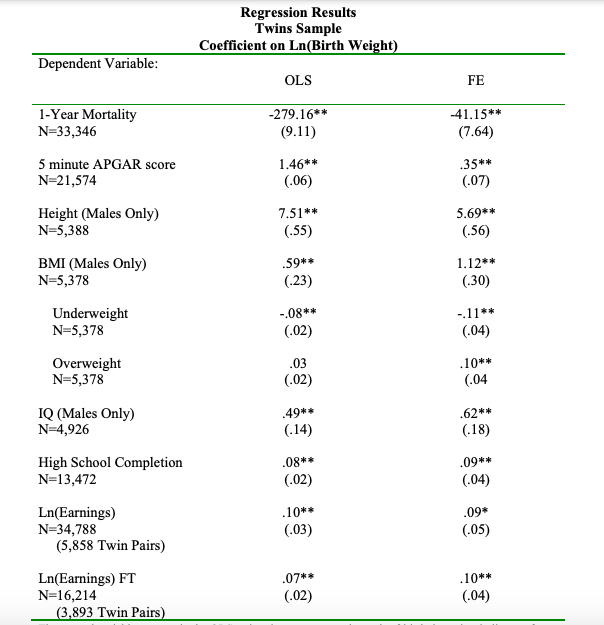
\includegraphics{black_results_nber.png}
\end{frame}

\begin{frame}{Problems that Fixed Effects Do Not Solve}
\protect\hypertarget{problems-that-fixed-effects-do-not-solve}{}
Consider the following regression model:

\[y_{it}=\mathbf{x}_{it}\mathbf{\beta}+c_i+\varepsilon_{it}\] where
\(y_{it}\) is murder rate and \(\mathbf{x}_{it}\) is police spending per
capita

What happens when we regress y on x and city fixed effects?

\begin{itemize}
\tightlist
\item
  \(\hat{\mathbf{\beta}}_{FE}\) is inconsistent unless strict exogeneity
  conditional on \(c_i\) holds
\item
  Implies \(\varepsilon_{it}\) is uncorrelated with past, current and
  future regressors
\end{itemize}

\vfill

Most common violations:

\begin{enumerate}
\tightlist
\item
  Time-varying omitted variables
\item
  Simultaneity
\end{enumerate}

\vfill

Fixed effects do not obviate need for good research design!

\vfill
\end{frame}

\begin{frame}{Fixed Effects and Differences-in-Differences}
\protect\hypertarget{fixed-effects-and-differences-in-differences}{}
``Diff-in-Diff'' is a common panel technique used for identification.

\vfill

In the basic setup, we have:

\begin{itemize}
\tightlist
\item
  Two periods, \(pre\) and \(post\), where post period identified by the
  dummy variable, \(Post_t\)
\item
  Two groups, Treatment and Control, where the treatment group
  identified by the dummy variable, \(Treat_i\) .
\end{itemize}

\vfill
\end{frame}

\begin{frame}{Fixed Effects and Differences-in-Differences}
\protect\hypertarget{fixed-effects-and-differences-in-differences-1}{}
Diff-in-Diff Specification:

\[y_{it}=\beta_0+\beta_1Post_t + \beta_2 Treat_i + \delta Post_t \times Treat_i + \varepsilon_{it}\]

\begin{itemize}
\tightlist
\item
  \(\delta\) is the differences-in-differences''estimator.
\item
  It is also called an ``average treatment effect''
\end{itemize}

\vfill
\end{frame}

\begin{frame}{Where does the term ``diff-in-diff'' come from?}
\protect\hypertarget{where-does-the-term-diff-in-diff-come-from}{}
``Diff-in-Diff'' takes two differences:

\begin{enumerate}
\tightlist
\item
  Pre vs Post
\item
  Treatment vs Control
\end{enumerate}

\[y_{it}=\beta_0+\beta_1Post_t + \beta_2 Treat_i + \delta Post_t \times Treat_i + \varepsilon_{it}\]

Write out predictions, their difference, then the difference in
differences:

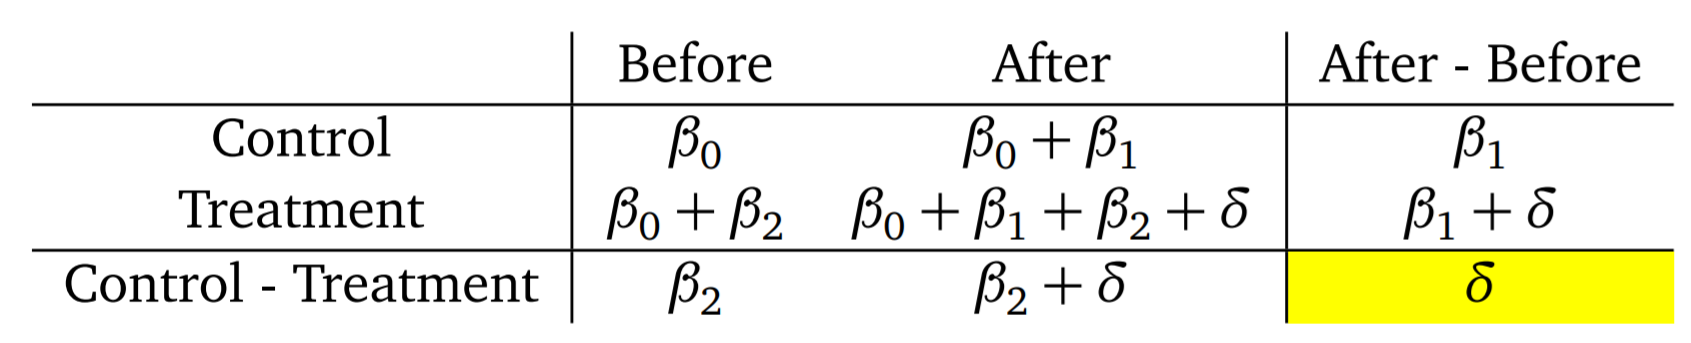
\includegraphics{Diff_Diff.png}

\vfill
\end{frame}

\begin{frame}{Where does the term ``diff-in-diff'' come from?}
\protect\hypertarget{where-does-the-term-diff-in-diff-come-from-1}{}
We have the ``diff-in-diff'' specification below:

\[y_{it}=\beta_0+\beta_1Post_t + \beta_2 Treat_i + \delta Post_t \times Treat_i + \varepsilon_{it}\]

\vfill

Treatment group might naturally differ from control: \(\beta_2\)

\vfill

Post might naturally differ from Pre: \(\beta_1\)

\vfill

Getting rid of both yields \(\delta\), the average treatment effect

\vfill
\end{frame}

\begin{frame}{Diff-Diff Identifying Assumption}
\protect\hypertarget{diff-diff-identifying-assumption}{}
The assumption for identification of the average treatment effect from
\(\delta\) is: \emph{in the absence of a real treatment, control and
treated units would have followed the same trends}.

\vfill

This assumption is called ``\textbf{the common trends assumption}'' or
``\textbf{the parallel trends assumption}

\vfill

It is untestable by definition.

\vfill

An important implication is that treated and untreated units need no to
be the same before policy adoption.

\vfill
\end{frame}

\begin{frame}{Diff-Diff Identifying Assumption}
\protect\hypertarget{diff-diff-identifying-assumption-1}{}
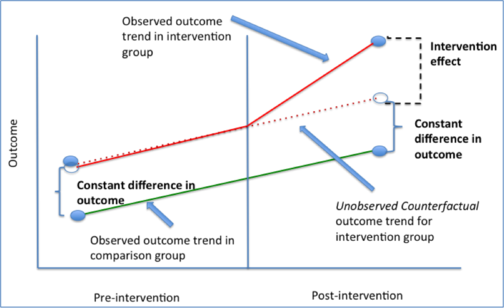
\includegraphics{DIDgraph.png}
\end{frame}

\begin{frame}{Threats to DID Assumptions}
\protect\hypertarget{threats-to-did-assumptions}{}
There are several reasons why the parallel assumption could fail:

\begin{itemize}
\tightlist
\item
  Lack of parallel trends
\item
  Differential attrition in treated and untreated units, which may lead
  to compositional changes.
\end{itemize}

\vfill

It is impossible to test the common trends assumptions, but:

\begin{itemize}
\tightlist
\item
  We can check pre-trends
\item
  If trends are similar before policy, then they would likely have
  continued to be similar in the post-period absent a real treatment.
\item
  Hence, it is important to have several periods before policy to really
  convince about the plausibility of the identifying assumption.
\end{itemize}

\vfill
\end{frame}

\begin{frame}{A More General DID Framework}
\protect\hypertarget{a-more-general-did-framework}{}
In practice, we have more than two periods, although the treatment
occurs after a given date.

\vfill

The identifying assumption could be valid conditional on certain
variables

\vfill

It could be interesting to include both time and unit fixed effects.

\vfill

So, a more general Diff-in-Diff specification is:

\[y_{it}=\beta_0+\delta Post_t \times Treat_i + \beta_1 \mathbf{X}_{it} + \lambda_i + t_t + \varepsilon_{it}\]
where \(\lambda_i\) are unit fixed effects and \(t_t\) are time fixed
effects.

\vfill
\end{frame}

\begin{frame}{Event-Study Specifications and Assumption in DID}
\protect\hypertarget{event-study-specifications-and-assumption-in-did}{}
How to check for pre-trends to convincingly evaluate the parallel trends
assumption?

\vfill

Estimate the differences-in-differences for each period before and after
policy adoption:

\[y_{it} = \beta_0 + \sum\delta_k^{pre}D_k^{pre}\times Treat_i + \sum\delta_k^{post}D_k^{post}\times Treat_i + \lambda_i + t_t + \varepsilon_{it}\]

If the identifying assumption is valid, then \(\delta_k^{pre} = 0\) for
all \(k\) before policy adoption

\vfill

That is, the trends before policy are the same.
\end{frame}

\begin{frame}{Other Important Extensions in DID}
\protect\hypertarget{other-important-extensions-in-did}{}
Differences-in-Differences do not need to be \emph{only} differences
between units over time

\vfill

Interesting applications use differences within and between different
groups.

\begin{itemize}
\tightlist
\item
  Examples: Differences between black and white in different states or
  countries
\end{itemize}

\vfill

There may be more comparison groups and implement
differences-in-differences-in-differences:

\begin{itemize}
\tightlist
\item
  Comparison between black and white in different states or countries
  before and after policy adoption
\end{itemize}

\vfill
\end{frame}

\begin{frame}{}
\protect\hypertarget{section}{}
Duflo (2001). \emph{Schooling and Labor Market Consequences of School
Construction in Indonesia: Evidence from an Unusual Policy Experiment.}
\textbf{American Economic Review}
\end{frame}

\begin{frame}{Question and Motivation}
\protect\hypertarget{question-and-motivation}{}
More school infraestructure, more schooling?

\vfill

Educational level in turns affect wages?

\vfill

What is the economic return to education?

\vfill
\end{frame}

\begin{frame}{Program Description}
\protect\hypertarget{program-description}{}
1973-1978: The Indonesian government built 61,000 schools equivalent to
one school per 500 children between 5 and 14 years old

\vfill

The enrollment rate increased from 69\% to 85\% between 1973 and 1978

\vfill

The number of schools built in each region depended on the number of
children out of school in those regions in 1972, before the start of the
program.

\vfill
\end{frame}

\begin{frame}{Treatment Effect Identification}
\protect\hypertarget{treatment-effect-identification}{}
There are 2 sources of variations in the intensity of the program for a
given individual:

\begin{enumerate}
\tightlist
\item
  \textbf{By region}: There is variation in the number of schools
  received in each region.
\item
  \textbf{By age}: Children who were older than 12 years in 1972 did not
  benefit from the program, whereas the younger a child was 1972, the
  more it benefited from the program --- because she spent more time in
  the new schools.
\end{enumerate}

\vfill

Sources of Data: 1995 population census. Individual-level data on:

\begin{enumerate}
\tightlist
\item
  Birth date
\item
  1995 salary level
\item
  1995 educational level
\end{enumerate}

\vfill
\end{frame}

\begin{frame}{A First Estimation of the Impact}
\protect\hypertarget{a-first-estimation-of-the-impact}{}
\textbf{Step 1}: Simplify the intensity of the program and the groups of
children affected by the program:

\begin{itemize}
\tightlist
\item
  High or low areas with school construction
\item
  Young cohort of children who benefited/Older cohort of children who
  did not benefit
\end{itemize}

\vfill
\end{frame}

\begin{frame}{Look at the Average Years of Schooling}
\protect\hypertarget{look-at-the-average-years-of-schooling}{}
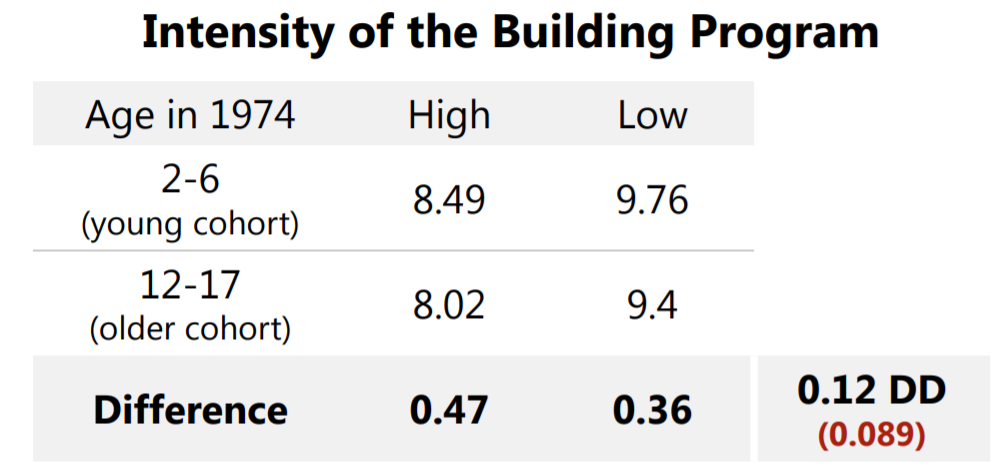
\includegraphics{duflo_simple_comparison.png}
\end{frame}

\begin{frame}{Placebo or Falsification Test}
\protect\hypertarget{placebo-or-falsification-test}{}
Idea: Look for 2 groups whom you know did not benefit, compute a DID,
and check whether the estimated effect is 0.

\vfill

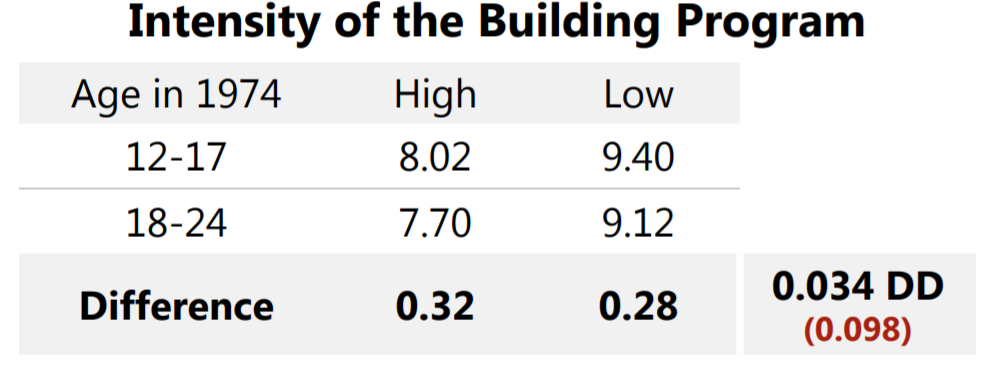
\includegraphics{duflo_simple_placebo.png}
\end{frame}

\begin{frame}{Formal Regression Results}
\protect\hypertarget{formal-regression-results}{}
\textbf{Step 2}:

\[S_{ijk} =  c + \alpha_j + \beta_k + \gamma P_j \times T_i + C_j \times T_i + \varepsilon_{ijk}\]

where:

\begin{itemize}
\tightlist
\item
  \(S_{ijk}\) educational level of the person \(i\) in region \(j\) in
  cohort \(k\)
\item
  \(P_j = 1\) if the person was born in a region with a high program
  intensity
\item
  \(T_i = 1\) if the person belongs to the ``young'' cohort
\item
  \(C_j\) dummy variable for region \(j\)
\item
  \(\beta_k\) cohort fixed effects
\item
  \(\alpha_j\) district of birth
\end{itemize}

\vfill

The key \textbf{differences-in-differences parameter} is \(\gamma\)

\vfill
\end{frame}

\begin{frame}{Formal Regression Results}
\protect\hypertarget{formal-regression-results-1}{}
\textbf{Step 3}: We will use the intensity of the program in each
region.

\vfill

We estimate the effect of the program for each cohort separately:

\[S_{ijk} =  c + \alpha_j + \beta_k + \sum_{i=2}^{23}{\gamma P_j \times d_i} + C_j \times T_i + \varepsilon_{ijk}\]

where \(d_i\) a dummy variable for belonging to cohort \(i\)

\vfill
\end{frame}

\begin{frame}{Program Effect per Cohort}
\protect\hypertarget{program-effect-per-cohort}{}
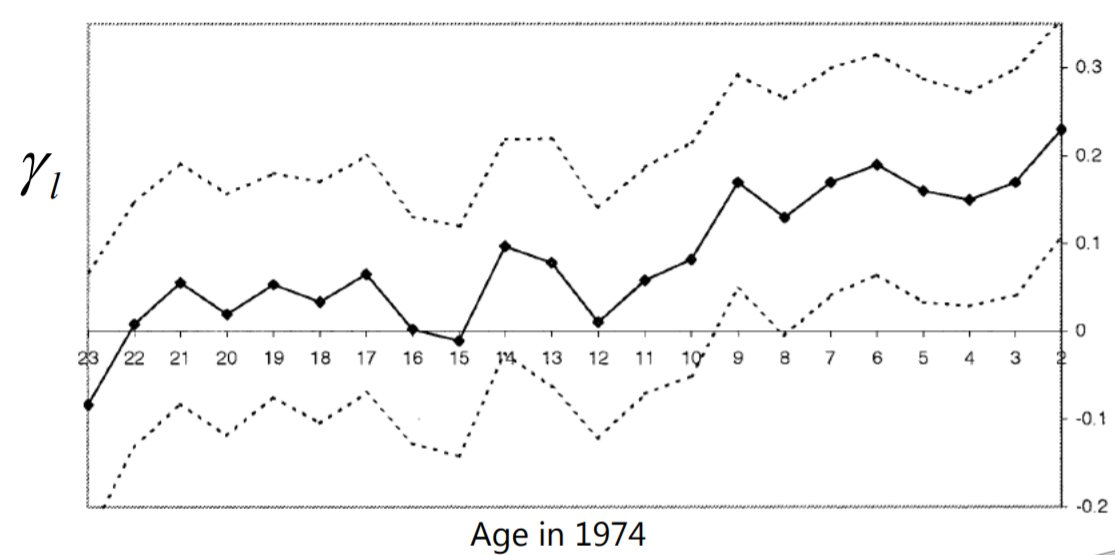
\includegraphics{duflo_effect_cohort.png}
\end{frame}

\begin{frame}{Effects on Salary}
\protect\hypertarget{effects-on-salary}{}
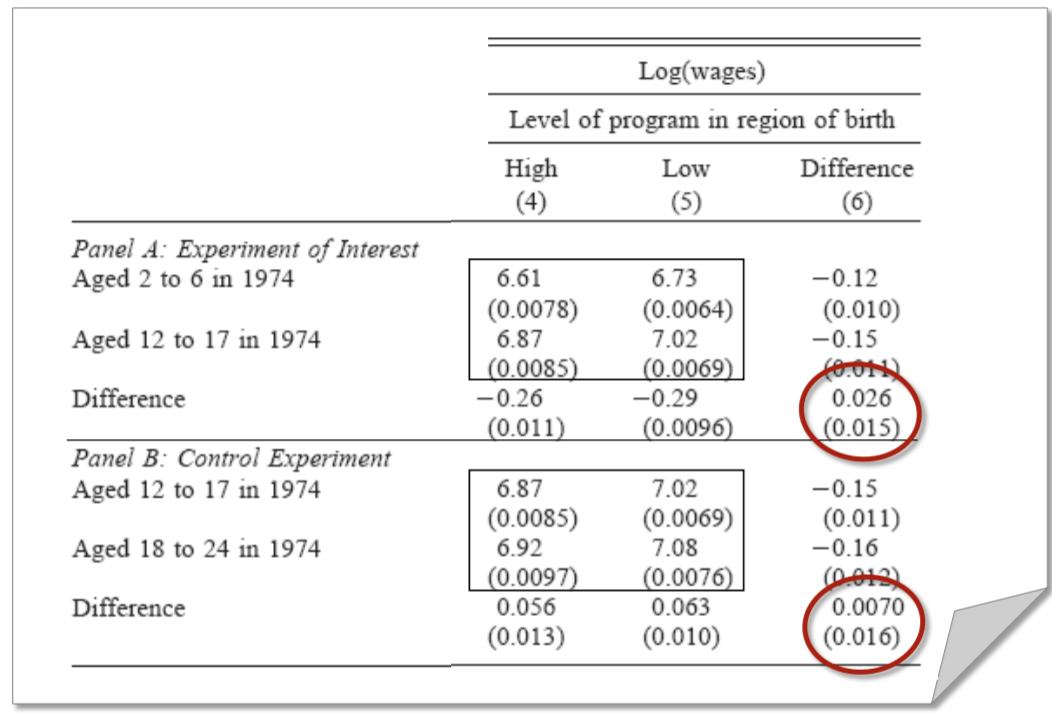
\includegraphics{duflo_salary.png}
\end{frame}

\begin{frame}{Conclusions}
\protect\hypertarget{conclusions}{}
Results: For each school built per 1000 students;

\begin{itemize}
\tightlist
\item
  The average educational achievement increase by 0.12-0.19 years
\item
  The average salaries increased by 2.6 -- 5.4\%
\end{itemize}

Making sure the DD estimation is accurate:

\begin{itemize}
\tightlist
\item
  A placebo DD gave 0 estimated effect
\item
  Use various alternative specifications
\item
  Check that the impact estimates for each age cohort make sense
\end{itemize}

\vfill
\end{frame}


\section[]{}
\frame{\small \frametitle{Table of Contents}
\tableofcontents}
\end{document}
